\chapter{{\LaTeX}\ Specific Usage}

This template is heavily built on \href{https://www.ctan.org/pkg/memoir}{memoir} package.
Check out memoir's documentation for its detailed usage and available customizations.

The thesis style is defined in the document class at \file{wustlthesis.cls}.
Since the school guideline is quite lenient, \texttt{wustlthesis} only contains minimal definition and has minimal required packages.
Packages that implement figures with multiple panels, table styling, hyperlinks, bibliography, and many other commonly used features are \emph{not} included in this document class.
You should feel free to use packages of your choice to enable those features.
Please check their compatibility with memoir through their documentations.

If you want to use the style of this thesis example, \file{thesis.tex} has some opinionated setup of the aforementioned features and you can find some showcases below.


\section{Figures}
Common file formats (PDF, PNG, and JPG) are supported.
Vector figures should be stored as PDF files to prevent pixelation.
For example, \fref{fig:vector} is a vector figure.

\begin{figure}[tb]
  \centering
  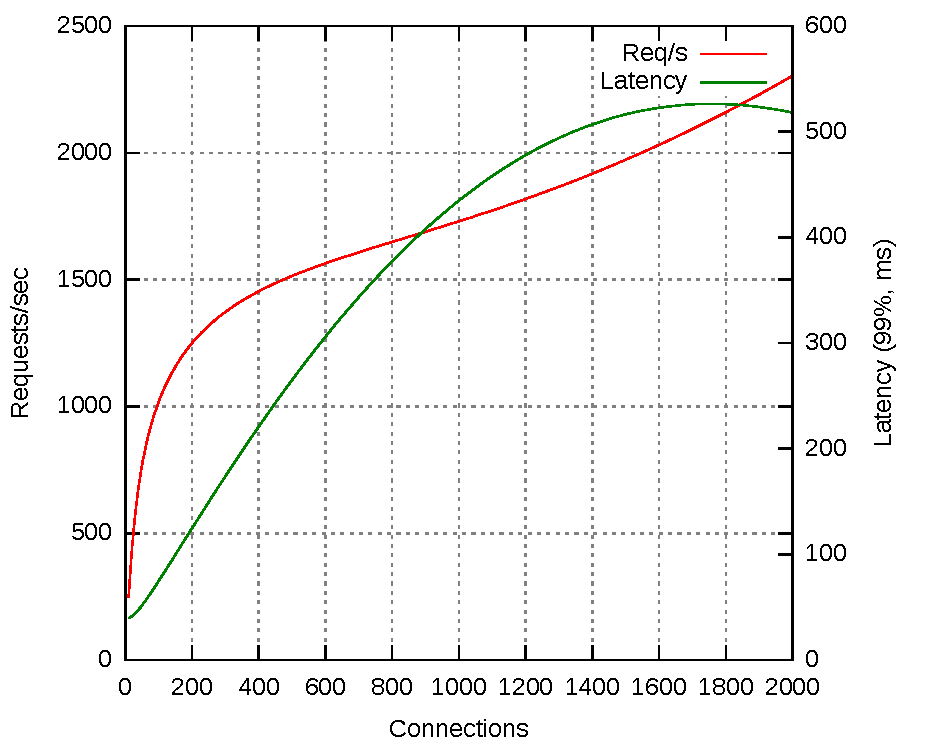
\includegraphics[width=0.6\textwidth]{figures/just-a-plot}
  \caption{Example vector figure in PDF.}
  \label{fig:vector}
\end{figure}



\section{Subfigures and subtables}
If a figure has multiple panels (subfigures), \texttt{subcaption} package is used to enable the correct references for subfigures.
Use \cmd{\fref}\marg{labstr} to refer to the full figure and \cmd{\fref}\marg{sublabstr} to refer to a specfic panel of that figure.
Use \cmd{\subcaptionref}\marg{sublabstr} to refer to just the panel number.
For example, \fref{fig:subfigure-demo} has two panels, \subcaptionref{fig:subfigdemo-cat} and \subcaptionref{fig:subfigdemo-dog}.
\fref{fig:subfigdemo-cat} refers to the cat panel.
This example explicitly creates the panel numbers since it is often to have figures with the panel numbers embedded.

\begin{figure}[t]
    \begin{subfigure}[b]{.5\linewidth}
        \centering
        \textbf{\sffamily A}\\[-0.5\onelineskip]
        \HUGE \emoji{cat}\\
        \emoji{cat-face}
        \phantomlabel{fig:subfigdemo-cat}
    \end{subfigure}%
    \begin{subfigure}[b]{.5\linewidth}
        \centering
        \textbf{\sffamily B}\\[-0.5\onelineskip]
        \HUGE \emoji{dog}\\
        \emoji{dog-face}
        \phantomlabel{fig:subfigdemo-dog}
    \end{subfigure}
    \caption[Two animals and their emojis.]{%
        Two animals and their emojis.
        \subref{fig:subfigdemo-cat} cats and \subref{fig:subfigdemo-dog} dogs.
    }
    \label{fig:subfigure-demo}
\end{figure}

Similarly, multiple tables can be grouped together as one using the same method. For example, see \tref{tab:subtable-demo}, which has two panels \subcaptionref{tab:subtab-a} and \subcaptionref{tab:subtab-b}.

\begin{table}[b]
    \centering
    \caption{Another table with two panels: \subref{tab:subtab-a} first and \subref{tab:subtab-b} second panel}
    \label{tab:subtable-demo}

    \begin{subtable}{0.5\linewidth}
        \centering
        \subcaption{First}\label{tab:subtab-a}
        \begin{tabular}{lc} \toprule
        A legendary table & 5 \\
        with two lines    & 6 \\ \bottomrule
        \end{tabular}
    \end{subtable}%
    \begin{subtable}{0.5\linewidth}
        \centering
        \subcaption{Second}\label{tab:subtab-b}
        \begin{tabular}{lc} \toprule
        A legendary table & 5 \\
        with two lines    & 6 \\ \bottomrule
        \end{tabular}
    \end{subtable}
\end{table}


\subsection{Figures with multiple panels merged into one source}
Sometimes the figure has already merges multiple panels and it's hard to split the panels into individual sources.
In this case, the panel numbers can be created using \cmd{\phantomlabel}\marg{labstr}.
For example, both \fref{fig:subfigure-demo} and \ref{fig:cell-cycle-mitosis} create panel numbers using this approach.


\subsection{Long figure legends spanning over the next page}
In some cases, the multi-panel figures may not have the vertical space to fit its legend, so the text overflow to the next page.
The text overflow can be achieved by using \cmd{\legendcontdnote} at the end of the first half of the legend (following the figure) and \cmd{\legendcontdref}\marg{labstr} at the beginning of the second half of the legend (usually at the next page).
\cmd{\legendcontdnote} inserts the ``\emph{(legend continued on next page)}'' mark right aligned at the end of the line or a new line.
\cmd{\legendcontdref} inserts the ``\emph{(Figure X continued)}'' mark.
Their style can modifyied by redefining the commands.

For example, \fref{fig:cell-cycle-mitosis} spans over two pages. Note how the two adjacent figure environments are constructed (and the figure placement specifier).

\begin{figure}[p]
    \centering
    \phantomlabel{fig:mitosis-prophase}
    \phantomlabel{fig:mitosis-prometaphase}
    \phantomlabel{fig:mitosis-metaphase}
    \phantomlabel{fig:mitosis-anaphase}
    \phantomlabel{fig:mitosis-telophase}
    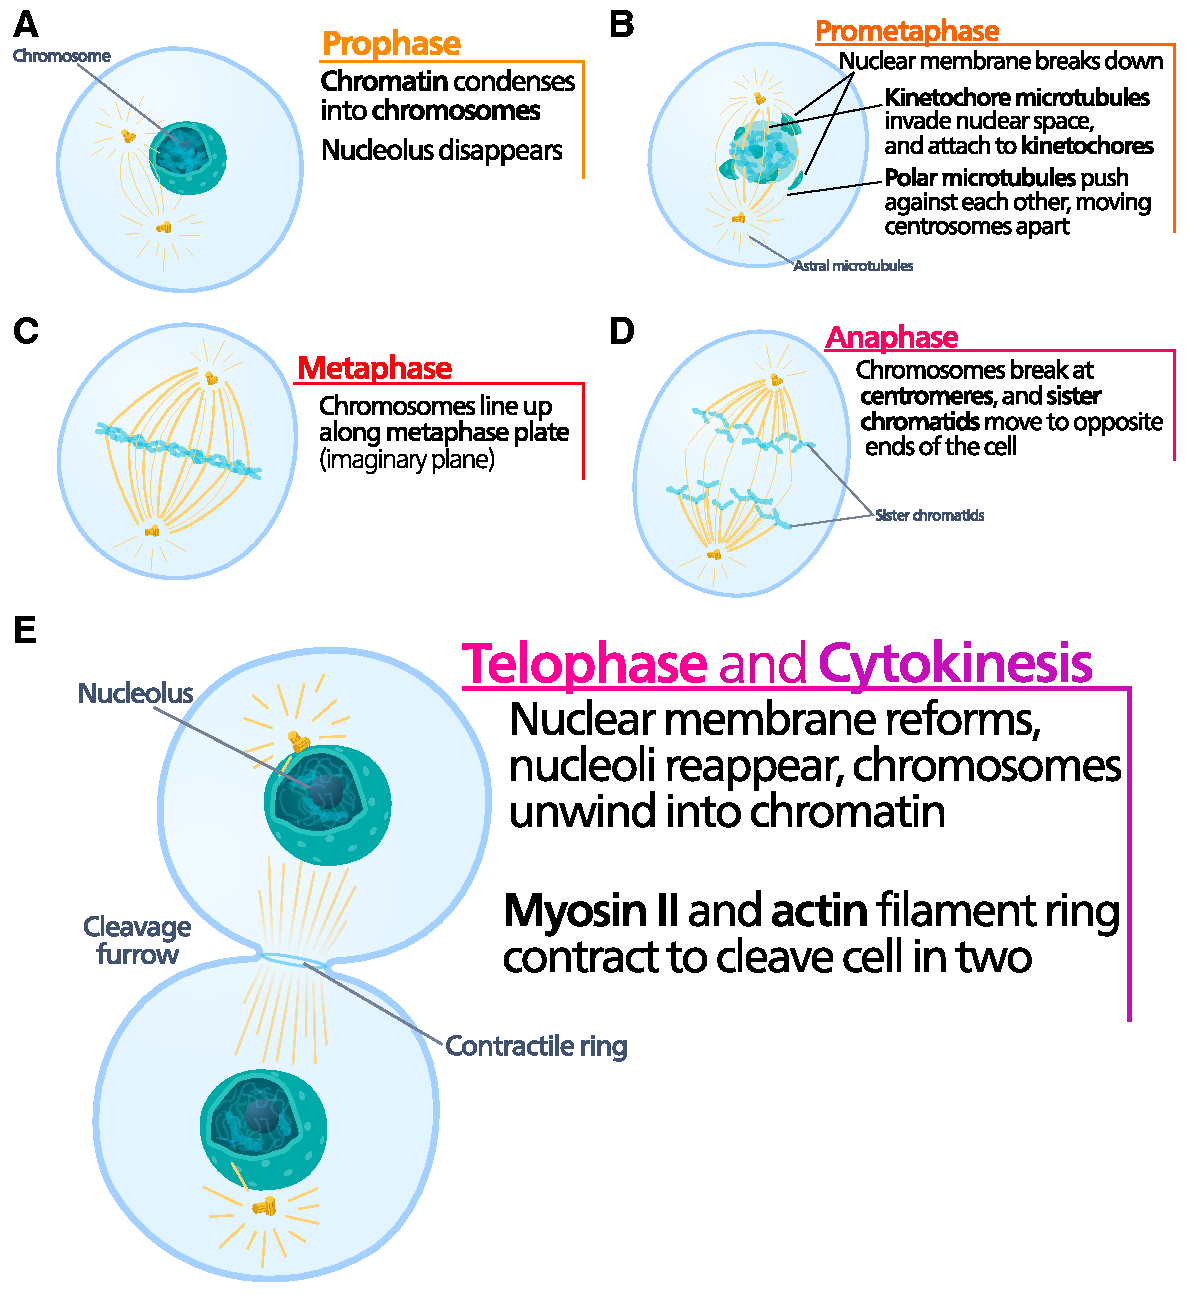
\includegraphics[width=\linewidth]{figures/cell-cycle-mitosis.pdf}
    \caption[Stages of mitotic phase of the cell cycle]{%
        Overview of different stages in the mitotic (M) phase of the animal cell cycle.
        Stages are defined based on the completion of a set of activities.
        \href{https://commons.wikimedia.org/wiki/File:Animal_cell_cycle-en.svg}{Figures} are made by Kelvin Ma (Kelvinsong; Kelvin13), \href{https://creativecommons.org/licenses/by/3.0}{CC BY 3.0}, via Wikimedia Commons.
        Text is copied from the \href{https://en.wikipedia.org/wiki/Mitosis}{Mitosis} page of Wikipedia.
        \subref{fig:mitosis-prophase}
        During prophase, which occurs after G\textsubscript{2} interphase,
        the cell prepares to divide by tightly condensing its chromosomes and initiating mitotic spindle formation.
        \subref{fig:mitosis-prometaphase}
        During prometaphase, the nuclear membrane breaks apart into numerous ``membrane vesicles'', and the chromosomes inside form protein structures called kinetochores.
        \legendcontdnote
    }
    \label{fig:cell-cycle-mitosis}
\end{figure}
\begin{figure}[t]
    \centering
    \legend{%
        \legendcontdref{fig:cell-cycle-mitosis}
        \subref{fig:mitosis-metaphase}
        During metaphase, the two centrosomes begin pulling the chromosomes towards opposite ends of the cell. The resulting tension causes the chromosomes to align along the metaphase plate or equatorial plane.
        \subref{fig:mitosis-anaphase}
        During anaphase, the replicated chromosomes are split and the newly-copied chromosomes are moved to opposite poles of the cell.
        \subref{fig:mitosis-telophase}
        During telophase, the effects of prophase and prometaphase (the nucleolus and nuclear membrane disintegrating) are reversed.
        Telophase is followed by cytokinesis, a separate process necessary for completing cell division.
    }
\end{figure}


\section{Tables}
While there are many packages for tabular environments, they should be compatible to this thesis document class.
Both examples (\tref{tab:include} and \ref{tab:nsf-sed}) use the \texttt{threeparttable} environment to format the table and allow table notes.
For more sophisticated formattings, check out the memoir documentation.

\begin{table}[tb]
    \centering
    \caption[Definite postgraduation commitments of doctorate recipients]{%
        Definite postgraduation commitments of doctorate recipients,
        by citizenship status and major field of study in 2019.
        Source: National Center for Science and Engineering Statistics, Survey of Earned Doctorates, National Science Foundation
        (\href{https://ncses.nsf.gov/pubs/nsf21308/}{link}; Table 51).
    }
    \label{tab:nsf-sed}
    \begin{threeparttable}[b]
    \begin{tabular}{llrrrrrrr@{}}
    \toprule
    Citizenship & Field & Total &
        Postdoc & Academia & Industry\tnote{a} & Other\tnote{b} & Abroad\\
    \midrule
    \multirow{3}{*}{\begin{tabular}[c]{@{}l@{}}All recipients\tnote{c}\end{tabular}}
        & Bio./biomed. & 5,054 &
            3,426 & 442 & 892 & 294 & 332 \\
        & Health & 1,525 &
            538	& 492 & 220 & 275 & 141\\
        & Comp./info. & 1,414 &
            276 & 254 & 789 & 95 & 161\\
    \midrule
    \multirow{3}{*}{\begin{tabular}[c]{@{}l@{}}U.S. citizen\\or PR\end{tabular}}
        & Bio./biomed. & 3,860 &
            2,536 & 385 & 679 & 260 & 118\\
        & Health & 1,248 &
            375 & 454 & 160 & 259 & 14\\
        & Comp./info. & 557 &
            102 & 133 & 247 & 75 & 23\\
    \midrule
    \multirow{3}{*}{\begin{tabular}[c]{@{}l@{}}Temporary\\visa holder\end{tabular}}
        & Bio./biomed. & 1,180 &
            882 & 55 & 212 & 31 & 213\\
        & Health & 275 &
            163 & 37 & 59 & 16 & 124\\
        & Comp./info. & 851 &
            173 & 120 & 540 & 18 & 136\\
    \bottomrule
    \end{tabular}
    \begin{tablenotes}
    \item[a] Includes doctorate recipients who indicated self-employment.
    \item[b] Includes doctorate recipients who indicated government, nonprofit, elementary or secondary school, or other employment and those with unknown employment.
    \item[c] Includes respondents who did not report citizenship status.
    \end{tablenotes}
    \end{threeparttable}
\end{table}


\section{Bibliography and Citations}
The \texttt{wustlthesis} document class does not implement any bibliography settings, so any tool stack should be compatible.

In this example, the bibliography is managed by \href{http://biblatex-biber.sourceforge.net/}{Biber} and \href{https://www.ctan.org/pkg/biblatex}{BibLaTeX} (not BibTeX), which support Unicode and more formatting options.
If \href{https://www.zotero.org/}{Zotero} is your reference manager, check out the \href{https://retorque.re/zotero-better-bibtex/}{Better BibTeX} plugin for Zotero to enable more seamless integration with BibLaTex (and BibTeX).

Regardless of the tool stack, the standard commands can be used for citations, e.g., \cmd{\cite}\marg{key} and \cmd{\citeauthor}\marg{key}.
For example, this paper by \citeauthor{Jinek2012} demonstrated CRISPR can cut DNA at specific nucleotide sequences \cite{Jinek2012}.


\section{Equations}
See Equation~\ref{eq:maxwell}.

\begin{equation}
    \label{eq:maxwell}
    \begin{aligned}
    \frac{\partial\mathcal{D}}{\partial t} & = \nabla\times\mathcal{H},   & \text{(Loi de Faraday)}\\
    \frac{\partial\mathcal{B}}{\partial t} & = -\nabla\times\mathcal{E},  & \text{(Loi d'Ampère)}\\
    \nabla\cdot\mathcal{B}                 & = 0,                         & \text{(Loi de Gauss)}\\
    \nabla\cdot\mathcal{D}                 & = 0.                         & \text{(Loi de Colomb)}
    \end{aligned}
\end{equation}

\clearpage
\section{Page layout}
\layout
